
                \begin{figure}
                    \centering
                    \begin{tikzpicture}
                        \pgfplotsset{%
                            width=1\textwidth,
                            height=0.4\textheight
                        }
                        \begin{axis}[
                            xlabel={Runs since restart},
                            ylabel={Average dynamic energy (watt)},
                            ymin=0,ymax=70,
                        ]
                        
                            \addplot [mark=none, densely dashed, red]  coordinates {
                            (1, 50.581959309218576)(2, 49.61038875471743)(3, 50.02540589470424)(4, 49.680261087585755)(5, 49.61474108469387)
                            };
                            \addlegendentry{WRK - IPG}
                            
                            \addplot [mark=none, densely dashed, blue]  coordinates {
                            (1, 50.05520471315441)(2, 49.53370095896579)(3, 50.05989598500499)(4, 50.19643007886517)(5, 50.02959293633925)
                            };
                            \addlegendentry{WRK - LHM}
                            
                            \addplot [mark=none, densely dashed, cyan]  coordinates {
                            (1, 44.8124775173346)(2, 40.2932455151716)(3, 36.20059282955928)(4, 41.23661828968479)(5, 44.91076231526205)
                            };
                            \addlegendentry{WRK - CLAMP (win)}
                            
                        \end{axis}
                    \end{tikzpicture} 
                \caption{A graph illustrating the energy consumption of Cores for test case BinaryTrees with regards to how long ago the DUT was restarted, experiment \#2, (without outliers)} \label{fig:BinaryTrees_Cores_iteration_exp2}
                \end{figure}
                